En los ejercicios de la siguiente sección utilizaremos el módulo \textbf{turtle} que se encuentra en Python. Cada ejercicio importará el módulo, así que presten atención a los ejemplos.

Además mencionar que utilizaremos una versión un poco diferente de lo que vimos en clases. En particular utilizaremos y definiremos la pantalla en la cual trabajaremos, así si observan el siguiente código:\\

\begin{listing}[H]
    \pythonblock{python/tortuga/tortugaBasica.py}
\end{listing}

Observamos lo siguiente:

\begin{itemize}
    \item Importamos los elementos usando \textbf{from turtle import Screen, Turtle}. Esto lo realizamos para importar solo esas funciones de la librería turtle (y no traernos todo). En caso de que necesitemos todo, el ejercicio nos dirá directamente \textbf{import turtle}.
    \item Creamos una pantalla a través de la función \textbf{Screen()} y definimos su tamaño utilizando la función \textbf{setup} (si necesitamos más grande o más chico acá vamos ajustando) de 425 píxeles de ancho y 225 píxeles de alto.
    \item En la línea \textbf{5} fijamos el tamaño de la superficie de dibujo en 400 píxeles de ancho y 200 píxeles de alto.
    \item A través de la función de la línea \textbf{7} controlamos que la pantalla de la tortuga se cierre una vez que demos clic sobre la interfaz
\end{itemize}

Entendiendo eso como esencial comenzamos con los ejercicios resueltos\footnote{Es recomendable comenzar a leer \href{https://docs.python.org/3/library/turtle.html}{documentación del módulo de turtle}}.

\begin{enumerate}[{Ejercicio} 1.]
    \item Diseñe un programa que dibuje un cuadrado por la pantalla de lado 100.\\
    
    \asw Para esto utilizaremos la función \textbf{fd} para mover nuestra tortuga 100 pasos hacia adelante y \textbf{rt} para girar a la derecha\footnote{\textbf{rt} es el nombre corto de \textbf{right}, al igual que \textbf{fd} es el nombre corto de \textbf{forward} o \textbf{lt} es de \textbf{left}}.\\

    \begin{listing}[H]
        \pythonblock{python/tortuga/cuadrado-turtle.py}
    \end{listing}

    El resultado debiese entregar esta figura\\

    \begin{figure}[H]
        \centering
        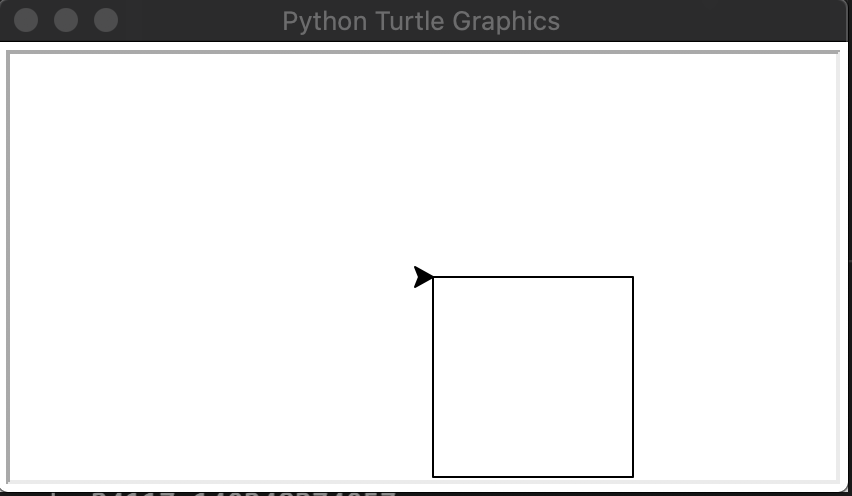
\includegraphics[scale=0.4]{cuadrado}
    \end{figure}

    \item Diseñe un programa que dibuje en la pantalla un triángulo equilátero de lado 100.\\
    
    \asw Para que sea un triángulo equilátero, todos sus lados miden lo mismo y los ángulos interiores son de \(60\degree\). Para esto usamos la función \textbf{lt} para hacer el triángulo hacia arriba. Además consideramos pasar \(120\) como valor a la función \textbf{lt} (diferencia entre 180 - 60). Así el código nos queda como:\\

    \begin{listing}[H]
        \pythonblock{python/tortuga/triangulo-turtle.py}
    \end{listing}

    Luego deberíamos ver por pantalla:

    \begin{figure}[H]
        \centering
        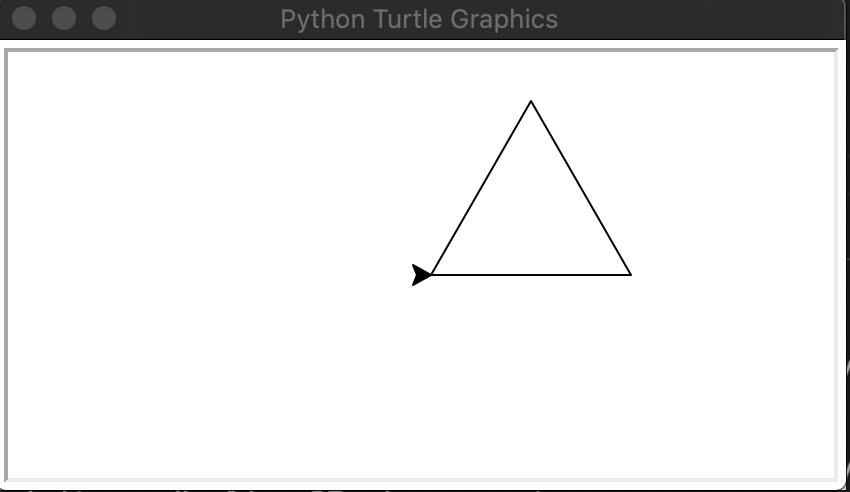
\includegraphics[scale=0.4]{triangulo}
    \end{figure}

    \item Diseñe un programa que dibuje un cuadrado cuyos lados midan 200 pasos y otro cuadrado cuyos lados midan 100 centrado al interior del cuadrado más grande.
    
    \asw Para esto usaremos \textbf{up} y \textbf{down} que levantan el pincel y lo bajan respectivamente. Con esto podemos mover libremente la tortuga sin pintar sobre el lienzo.

    Para posicionar a la tortuga dentro del cuadrado grande, levantaremos el pincel y nos moveremos 50 pasos hacia el frente y 50 pasos hacia abajo. Una vez en esa posición dibujaremos el segundo cuadrado y nos quedará centrado. Así el código quedaría:\\

    \begin{listing}[H]
        \pythonblock{python/tortuga/inception-cuadrado-turtle.py}
    \end{listing}

    Y obtendremos como resultado la siguiente figura:\\

    \begin{figure}[H]
        \centering
        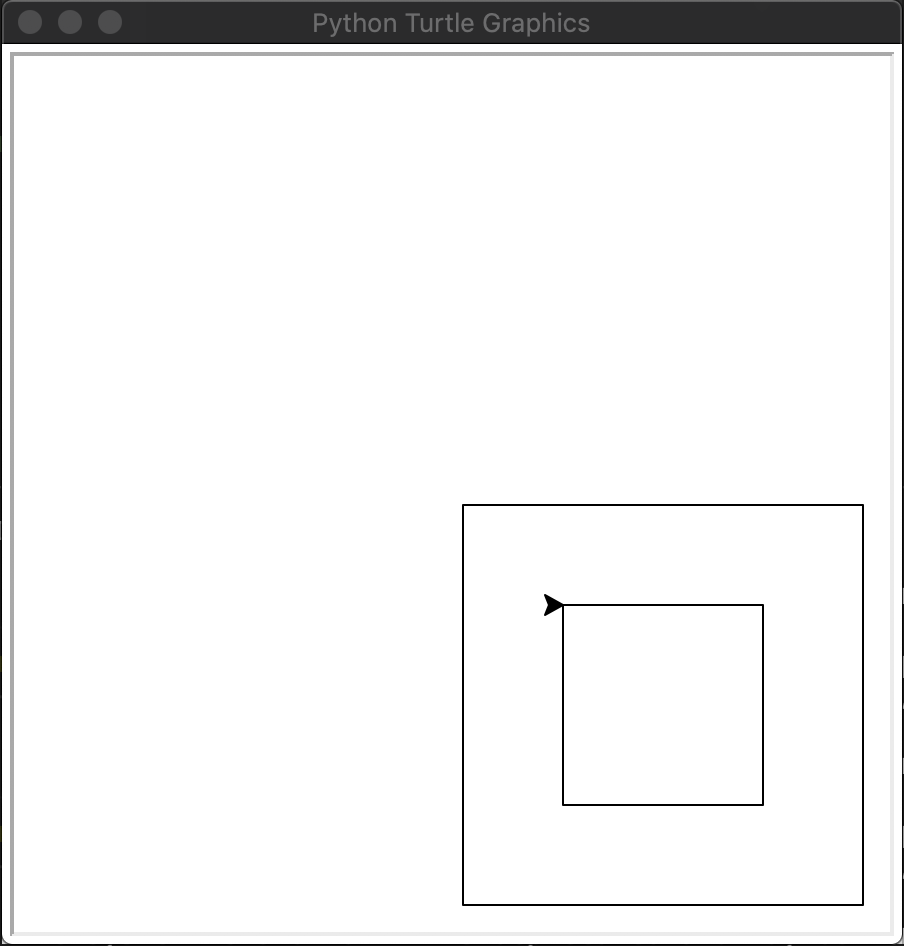
\includegraphics[scale=0.4]{cuadrado-inception}
    \end{figure}

    \item Diseñar un programa que permita visualizar un gráfico de torta a través de la aplicación \textbf{turtle} en donde exista la siguiente distribución de porcentajes: suspensos 10\%, 20\% de aprobados, un 40\% de notables y un 30\% de sobresalientes.\\
    
    \asw Para desarrollar este programa, lo realizaremos paso a paso. Lo primero que se realizará es el círculo de nuestro gráfico de torta. Para esto definiremos una circunferencia de radio 300. Moveremos el pincel desde la posición \textit{(0,0)} a la posición \textit{(0,-300)} para dejar un gráfico centrado en la ventana.\\

    \begin{listing}[H]
        \pythonblock{python/tortuga/pastel-1.py}
    \end{listing}

    Con esto tendremos una imagen de este tipo:\\

    \begin{figure}[H]
        \centering
        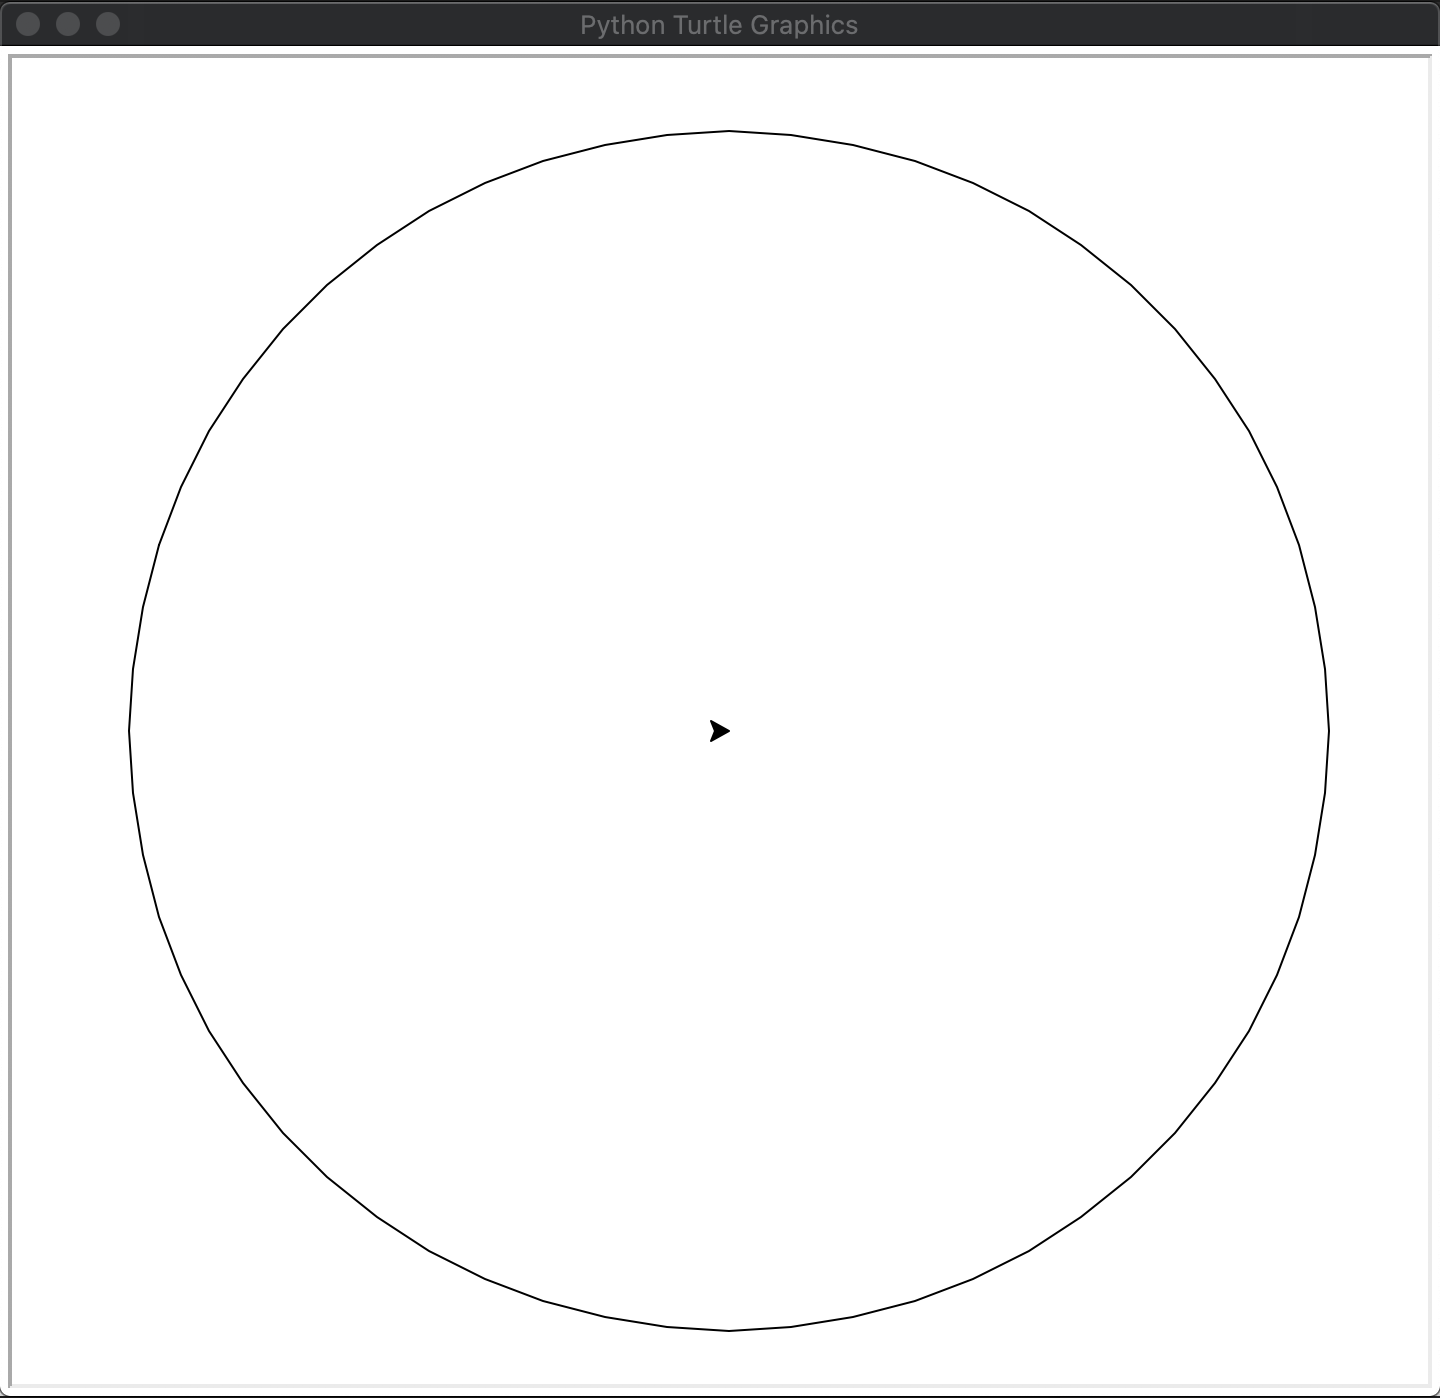
\includegraphics[scale=0.4]{circulo-1}
    \end{figure}

    Con la función \textbf{tortuga.home()} movemos al pincel a la posición inicial \textit{(0,0)}. Al levantar y bajar el pincel a conveniencia podemos graficar el círculo sin graficar todos los movimientos de éste al moverlo a los puntos de inicio del dibujo de la circunferencia.

    Guardamos las calificaciones en variables y agregamos comentarios para mayor claridad de nuestro código, así el código nos quedaría de la siguiente forma:\\

    \begin{listing}[H]
        \pythonblock{python/tortuga/pastel-2.py}
    \end{listing}

    Luego si queremos dibujar las líneas divisoras de las calificaciones, tendremos que calcular los ángulos necesarios de cada una de las calificaciones. Para esto usaremos la fórmula:

    \[ angulo_{calificacion} = \frac{360 * tipo_{nota}}{100} \]

    Así haciendo el lineamiento por cada uno de los porcentajes de notas, tenemos el siguiente código:\\

    \begin{listing}[H]
        \pythonblock{python/tortuga/pastel-3.py}
    \end{listing}

    \setcounter{pythonnumber}{40}

    \begin{listing}[H]
        \pythonblock{python/tortuga/pastel-31.py}
    \end{listing}

    Acá observamos también la función \textbf{write} que nos permite escribir un texto en el gráfico. Así nos quedaría el gráfico de la siguiente manera:\\

    \begin{figure}[H]
        \centering
        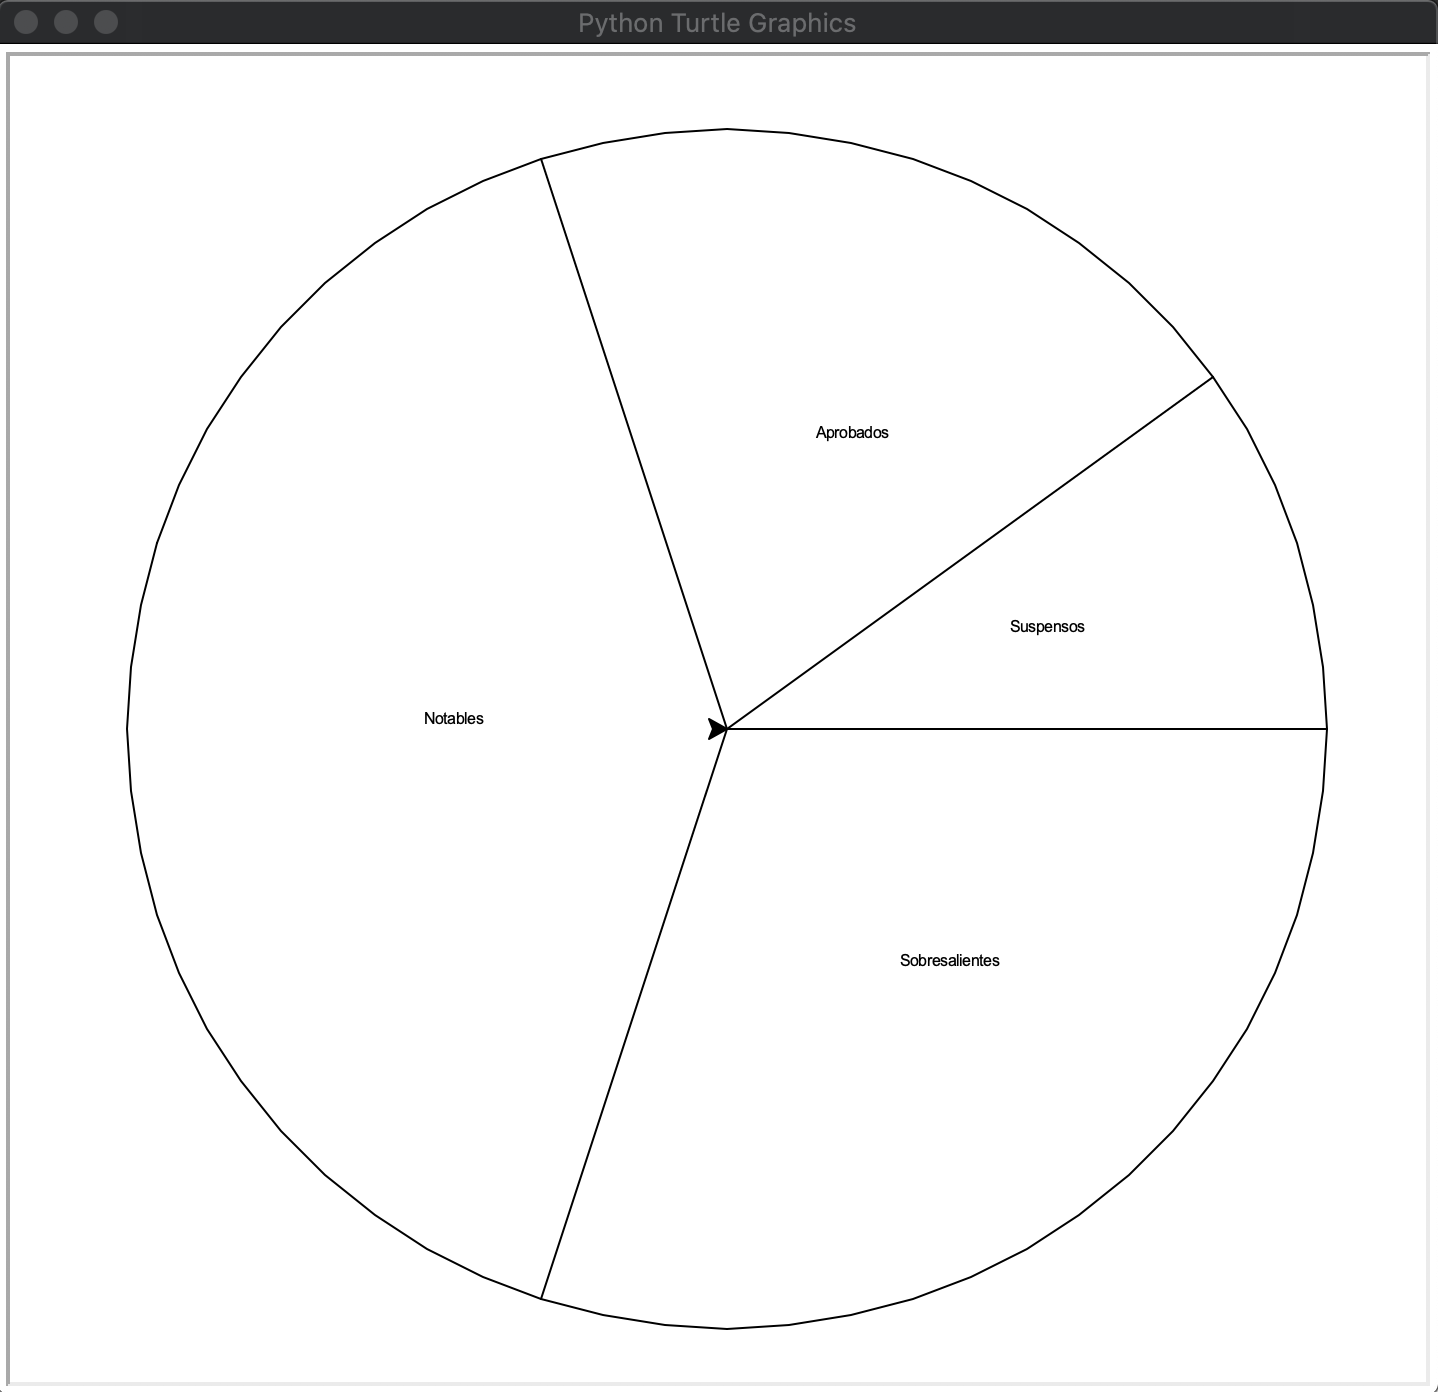
\includegraphics[scale=0.4]{circulo-3}
    \end{figure}

    \setcounter{pythonnumber}{1}

\end{enumerate}